\documentclass{beamer}
\usetheme{metropolis}
\usepackage{graphicx}
\usepackage{amsmath}
\usepackage{tcolorbox}
\title{Digital Signal Processing: COSC390}
\author{Jordan Hanson}
\institute{Whittier College Department of Physics and Astronomy}

\begin{document}
\maketitle

\begin{frame}{Normal distribution}
\textbf{Normally distributed} data decreases in probability at a rate that is proportional (1) to the \textit{distance from the mean}, and that is proportional (2) to the \textit{probability itself.}
\begin{figure}
\centering
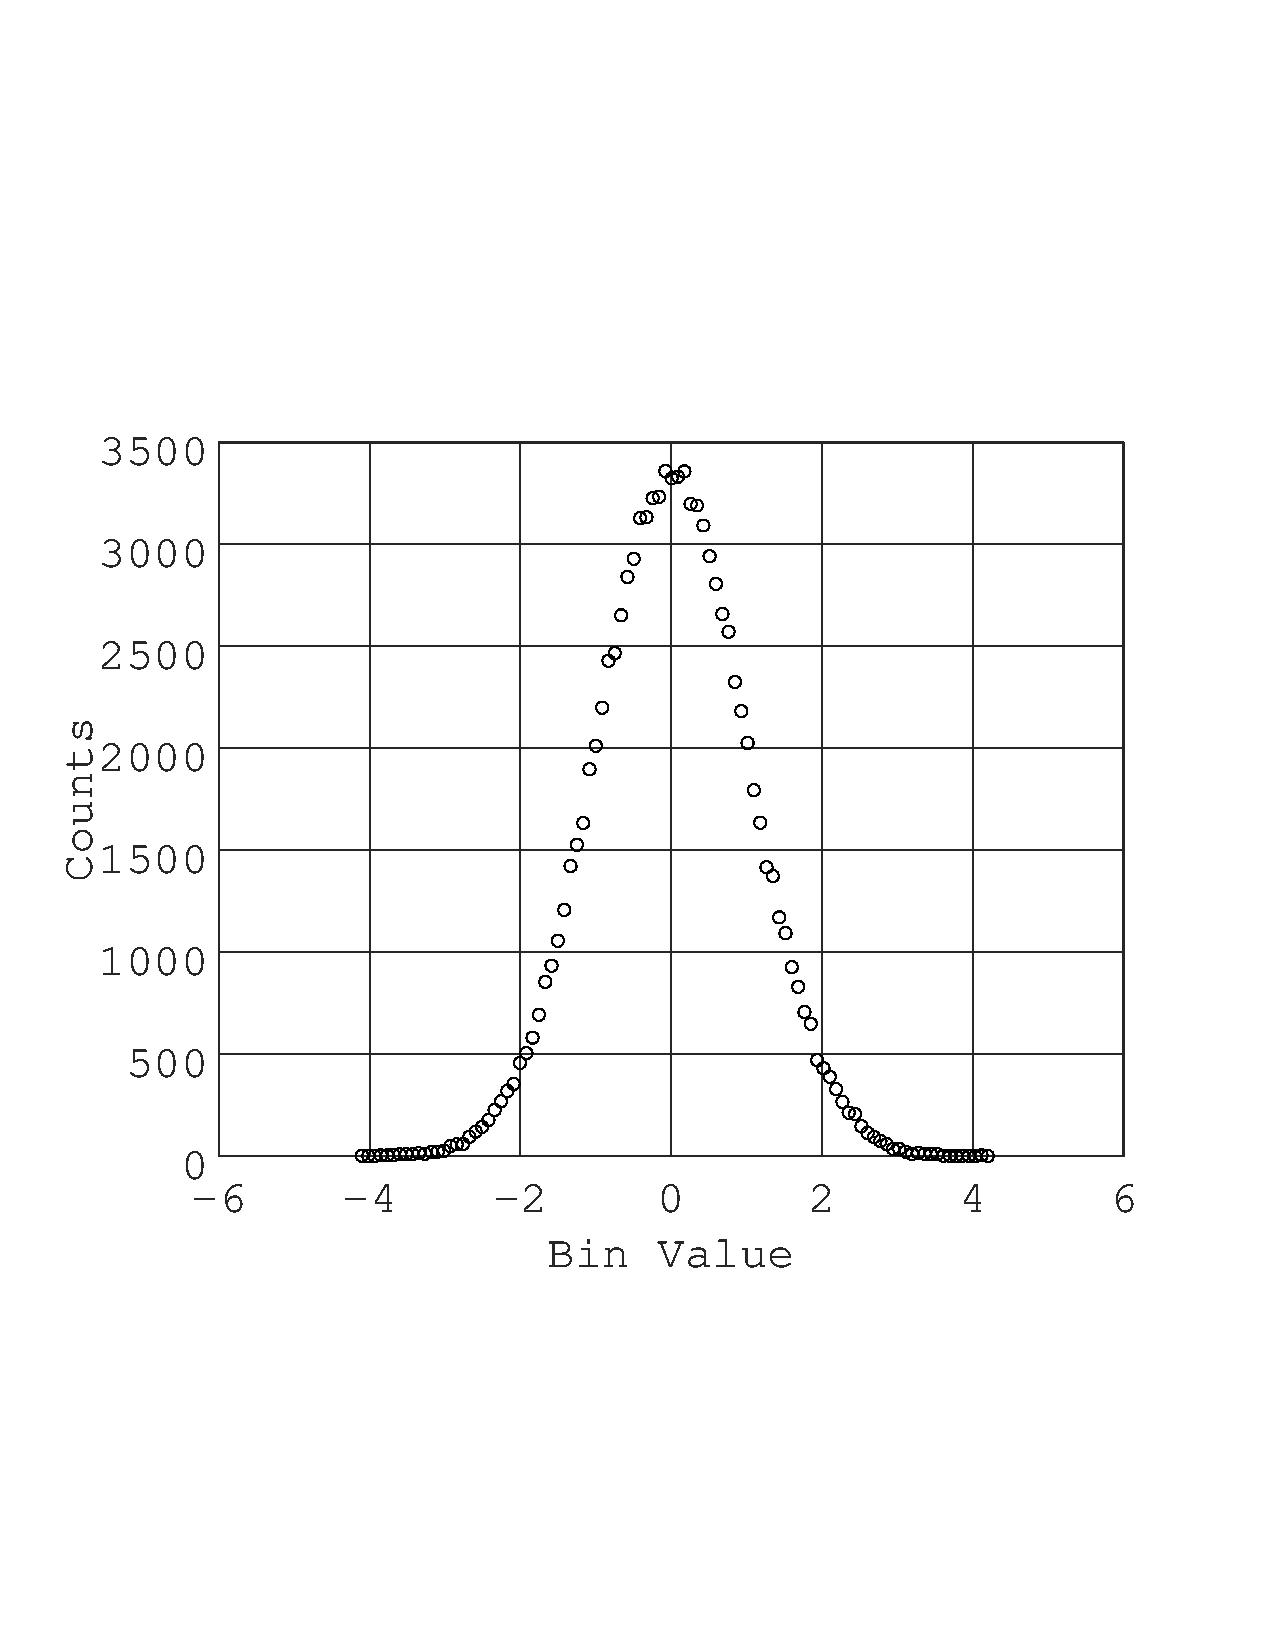
\includegraphics[width=0.5\textwidth,trim=0cm 6cm 0cm 6cm,clip=true]{figures/hist_binCount.pdf}
\caption{\label{fig:hist1} Normally distributed data counts decrease as measured further from the mean for \textit{two reasons.}}
\end{figure}
\end{frame}

\begin{frame}{Normal distribution}
\begin{tcolorbox}[colback=white,colframe=red!40!blue,title=Normal Distribution PDF]
Let $p(x)$ be the PDF of normally distributed data $x$ with mean $\mu$. In order to obey conditions (1) and (2), the function $p(x)$ must be described by the following differential equation, where $k$ is some constant.
\alert{\begin{equation}
\frac{dp}{dx} = -k(x-\mu)p(x) \label{eq:normDiffeq}
\end{equation}}
\end{tcolorbox}
\end{frame}

\begin{frame}{Normal distribution}
Rearranging Eq. \ref{eq:normDiffeq}, we have
\begin{equation}
\frac{dp}{p} = -k(x-\mu) dx
\end{equation}
Integrating both sides gives
\begin{equation}
\ln(p) = -\frac{1}{2}k(x-\mu)^2+C_0
\end{equation}
Exponentiating,
\begin{equation}
p(x) = C_1 \exp\left(-\frac{1}{2}k(x-\mu)^2\right) \label{eq:normDiffeq2}
\end{equation}
Ensuring that the PDF is \textit{normalized} requires
\begin{equation}
\int_{-\infty}^{\infty} p(x) dx = 1
\end{equation}
\end{frame}

\begin{frame}{Normal distribution}
But how do we integrate Eq. \ref{eq:normDiffeq2}?  First, a change of variables.  Let $s = x-\mu$
\end{frame}

\end{document}
